%!TEX TS-program = xelatex
%!TEX encoding = UTF-8 Unicode

\documentclass[12pt]{extarticle}
% extarticle is like article but can handle 8pt, 9pt, 10pt, 11pt, 12pt, 14pt, 17pt, and 20pt text

\def \ititle {Origins of Mind}
 
\def \isubtitle {Lecture 07}
 
\def \iauthor {Stephen A. Butterfill}
\def \iemail{s.butterfill@warwick.ac.uk}
\date{}

%for strikethrough
\usepackage[normalem]{ulem}

\input{$HOME/Documents/submissions/preamble_steve_handout}

%\bibpunct{}{}{,}{s}{}{,}  %use superscript TICS style bib
%remove hanging indent for TICS style bib
%TODO doesnt work
\setlength{\bibhang}{0em}
%\setlength{\bibsep}{0.5em}


%itemize bullet should be dash
\renewcommand{\labelitemi}{$-$}

\begin{document}

\begin{multicols}{3}

\setlength\footnotesep{1em}


\bibliographystyle{newapa} %apalike

%\maketitle
%\tableofcontents




%--------------- 
%--- start paste

\def \ititle {Origins of Mind}
 
\def \isubtitle {Lecture 07}
 
 
 
\
 
 
 
\begin{center}
 
{\Large
 
\textbf{\ititle}: \isubtitle
 
}
 
 
 
\iemail %
 
\end{center}
 
 
 
\section{Core Knowledge}
 
For someone to have \textit{core knowledge of a particular principle or fact} is for her to have a core system where either the core system includes a representation of that principle or else the principle plays a special role in describing the core system.
 
\subsection{The idea}
 
‘We hypothesize that uniquely human cognitive achievements build on systems that humans share with other animals: core systems that evolved before the emergence of our species.
The internal functioning of these systems depends on principles and processes that are distinctly non-intuitive.
Nevertheless, human intuitions about space, number, morality and other abstract concepts emerge from the use of symbols, especially language, to combine productively the representations that core systems deliver’
\citep[pp.\ 2784-5]{spelke:2012_core}.
 
\subsection{Two-part definition}
 
‘Just as humans are endowed with multiple, specialized perceptual systems, so we are endowed with multiple systems for representing and reasoning about entities of different kinds.’
\citep[p.\ 517]{Carey:1996hl}
 
‘core systems are
largely innate,
encapsulated, and
unchanging,
arising from phylogenetically old systems
built upon the output of innate perceptual analyzers’
\citep[p.\ 520]{Carey:1996hl}.
 
\textit{Note} There are other, slightly different statements \citep[e.g.][]{carey:2009_origin}.
 
\subsection{Compare modularity}
 
Modules are ‘the psychological systems whose operations present the world to thought’; they ‘constitute a natural kind’; and there is ‘a cluster of properties that they have in common’ \citep[p.\ 101]{Fodor:1983dg}.
 
These properties include:
 
\begin{itemize}
 
\item domain specificity (modules deal with ‘eccentric’ bodies of knowledge)
 
\item limited accessibility (representations in modules are not usually inferentially integrated with knowledge)
 
\item information encapsulation (modules are unaffected by general knowledge or representations in other modules)
 
\item innateness (roughly, the information and operations of a module not straightforwardly consequences of learning; but see \citet{Samuels:2004ho}).
 
\end{itemize}
 
 
 
\section{Syntax / Innateness}
 
Is the syntactic structure of ‘the red ball’ (a) flat or (b) hierachical?
 
\begin{center}
 
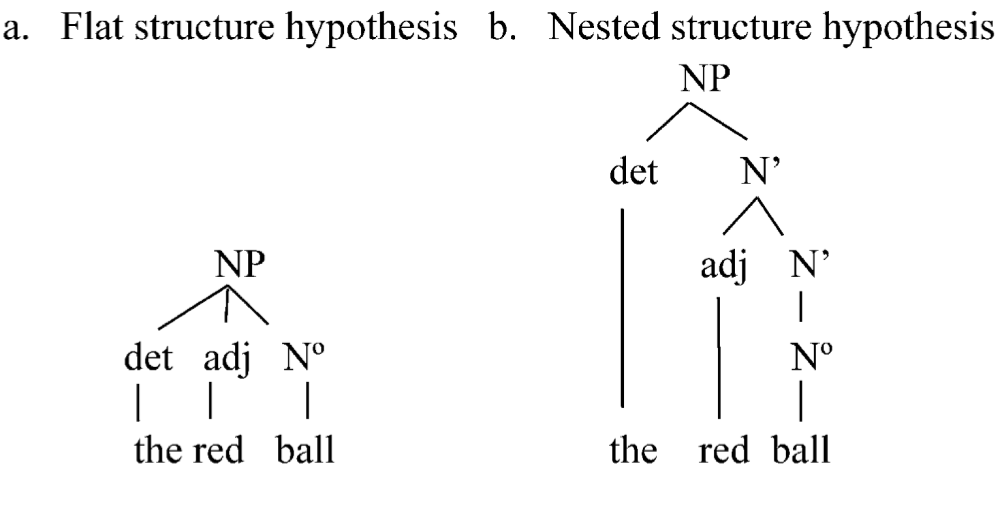
\includegraphics[scale=0.25]{../www.slides/src/raw/img/lidz_2003_fig0.neg.png}
 
\end{center}
 
\begin{center} from \citealp{lidz:2003_what} \end{center}
 
\begin{enumerate}
\item ‘red ball’ is a constituent on (b) but not on (a)
\item anaphoric pronouns can only refer to constituents
\item In the sentence ‘I’ll play with this red ball and you can play with that one.’, the word ‘one’ is an anaphoric prononun that refers to ‘red ball’ (not just ball). \citep{lidz:2003_what,lidz:2004_reaffirming}.
 
\end{enumerate}
 
‘The assumption in the preferential looking task is that infants prefer to look at an image that matches the linguistic stimulus, if one is available’ \citep{lidz:2003_what}.
 
\subsection{Poverty of stimulus arguments}
 
How do poverty of stimulus arguments work? See \citet{pullum:2002_empirical}.
 
\begin{enumerate}
 
\item
 
Human infants acquire X.
 
\item
 
To acquire X by data-driven learning you'd need this Crucial Evidence.
 
\item
 
But infants lack this Crucial Evidence for X.
 
\item
 
So human infants do not acquire X by data-driven learning.
 
\item
 
But all acquisition is either data-driven or innately-primed learning.
 
\item
 
So human infants acquire X by innately-primed learning .
 
\end{enumerate}
 
‘the APS [argument from the poverty of stimulus] still awaits even a single good supporting example’
\citep[p.\ 47]{pullum:2002_empirical}
 
 
 
\section{Pointing}
 
From around 11 or 12 months of age infants spontaneously point to request, inform and initiate joint engagement \citep{Liszkowski:2007mm}.
 
‘infant pointing is best understood---on many levels and in many ways---as depending on uniquely human skills and motivations for cooperation and shared intentionality, which enable such things as joint intentions and joint attention in truly collaborative interactions with others (Bratman, 1992; Searle, 1995).’
\citep[p.\ 706]{Tomasello:2007fi}
 
\subsection{Why don’t ape’s point?}
 
‘there is not a single reliable observation, by any scientist anywhere, of one ape pointing for another’.
\citep[p.\ 507]{Tomasello:2010dy}
 
‘Although some apes, especially those with extensive human contact, sometimes point imperatively for humans […],
 
no apes point declaratively ever.’
\citep[p.\ 510]{Tomasello:2010dy}
 
‘to understand pointing, the subject needs to understand more than the individual goal-directed behaviour. She needs to understand that by pointing towards a location, the other attempts to communicate to her where a desired object is located; that the other tries to inform her about something that is relevant for her’
\citep[p.\ 6]{Moll:2007gu}.
 
'the specific behavioral form---distinctive hand shape with extended index finger---actually emerges reliably in infants as young as 3 months of age (Hannan \& Fogel, 1987). [...] why do infants not learn to use the extended index finger for these social functions at 3 – 6 months of age, but only at 12 months of age?' \citep[p.\ 716]{Tomasello:2007fi}
 
Comprehending pointing is not just a matter of locking onto the thing pointed to; it also involves some sensitivity to context \citep[see][]{Liebal:2010lr}.
 
\subsection{Pointing: referent and context}
 
‘Already by age 14 months, then, infants interpret communication cooperatively, from a shared rather than an egocentric perspective’ \citep[p.\ 269]{Liebal:2010lr}.
 
‘The fact that infants rely on shared experience even to interpret others’ nonverbal pointing gestures suggests that this ability is not specific to language but rather reflects a more general social-cognitive, pragmatic understanding of human cooperative communication’ \citep[p.\ 270]{Liebal:2010lr}.
 
\subsection{pointing vs linguistic communication}
 
‘the most fundamental aspects of language that make it such a uniquely powerful form of human cognition and communication---joint attention, reference via perspectives, reference to absent entities, cooperative motives to help and to share, and other embodiments of shared intentionality---are already present in the humble act of infant pointing.’ \citep[p.\ 719]{Tomasello:2007fi}
 
‘cooperative communication does not depend on language, […] language depends on it.’ \citep[p.\ 720]{Tomasello:2007fi}
 
‘Pointing may […] represent a key transition, both phylogenetically and ontogenetically, from nonlinguistic to linguistic forms of human communication.’ \citep[p.\ 720]{Tomasello:2007fi}
 
 
 
\section{What is a communicative action?}
 
Theory of communicative action \citep[compare][]{Tomasello:2007fi}:
 
\begin{enumerate}
 
\item
 
Producing and understanding declarative pointing gestures constitutively involves embodying (?) shared intentionality.
 
\item
 
Embodying shared intentionality involves having knowledge about knowledge of your intentions about my intentions.
 
\end{enumerate}
 
\subsection{A Gricean view}
 
First approximation: To communicate is to provide someone with evidence of an intention with the further intention of thereby fulfilling that intention
\citep[compare][chapter 14]{Grice:1989ha}.
 
\subsection{First alternative view}
 
‘No speaker needs to form any express intention … in order to mean by a word what it means in the language’
\citep[p.\ 473]{Dummett:1986mq}
 
‘Interpreting speech does not require making any inferences or having any beliefs about words, let alone about speaker intentions’
\citep[p.\ 62]{Millikan:1984ib}
 
\subsection{Davidsonian view}
 
‘meaning of whatever sort ultimately rests on intention’
\citep[p.\ 298]{Davidson:1992pl}
 
ulterior intentions: ‘intentions which lie as it were beyond the production of words … [such as] the intention of being elected mayor, of amusing a child, of warning a pilot of ice on the wings’ \citep[p.\ 298]{Davidson:1992pl}.
 
semantic intentions: intentions concerning the meaning of one’s utterance.
 
‘The intention to be taken to mean what one wants to be taken to mean is, it seems to me, so clearly the only aim that is common to all verbal behaviour that it is hard for me to see how anyone can deny it.’
\citep[p.\ 11]{Davidson:1994ol}
 
 
 
%--- end paste
%--------------- 
 
\footnotesize 
\bibliography{$HOME/endnote/phd_biblio}

\end{multicols}

\end{document}